%INICIO DE CAPITULO
\chapter{FUNDAMENTAÇÃO TEÓRICA}
\label{cap:2}
\thispagestyle{empty}

Apresente um resumo das teorias utilizadas de forma a facilitar o acesso ao leitor do trabalho aos pré-requisitos para o entendimento do trabalho.

\section{Teoria dos Registros das Representações Semióticas}
\label{3.1}

 Ensinar é uma tarefa ...
O psicólogo e filósofo Raymond Duval, desenvolveu a Teoria dos Registros de Representação Semiótica - (TRRS)... 

A \emph{conversão} para \citeonline{colombo2008} é (exemplo de citação):

\begin{citacao}
 [...] a conversão de uma representação se refere às operações em que o registro inicial é transformado em outro registro; por essa razão, é considerada como uma “transformação externa”. Por exemplo, ao utilizarmos a linguagem algébrica para representar a frase “o dobro de um número resulta em oito”, estamos realizando uma conversão do registro dado na língua natural para o registro dado na linguagem algébrica \cite[p. 6]{colombo2008}.
\end{citacao}

Exemplo de figura.

\BFIG{Representação gráfica da função afim}

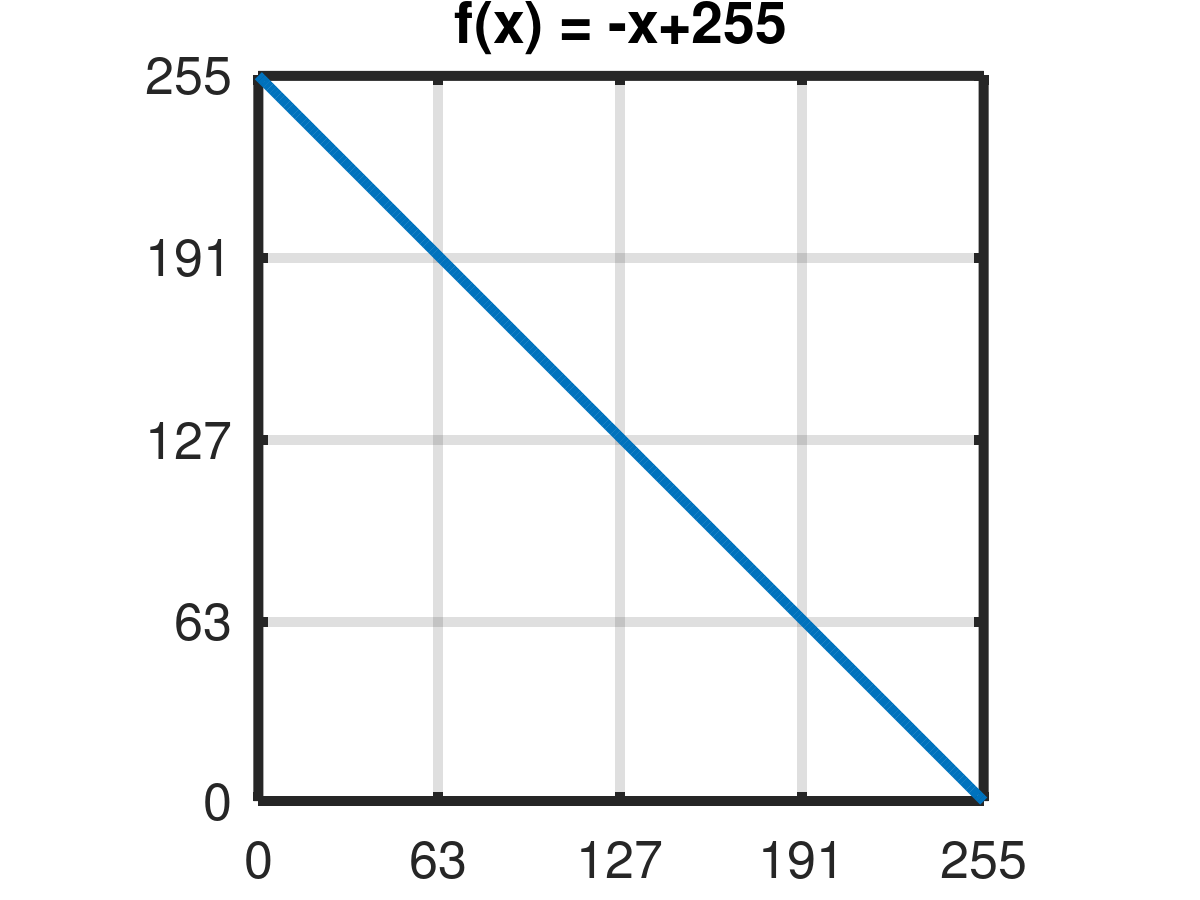
\includegraphics[width=0.60\linewidth]{./figuras/funcao.png}

\EFIG{Fonte: Elaborada pelo autor }{fig:repre}

Assim, a Figura \ref{fig:repre}..
	


\section{Exemplo de seção.}
\label{sec:introfunc}

\citeonline[p. 81]{murakami2004iezzi}, define Função como: 

\begin{definicao} 
Dado dois conjuntos $A$ e $B$, não vazios, uma relação $f$ de $A$ em $B$ recebe o nome de aplicação de $A$ em $B$ ou função definida em $A$ com imagens em $B$ se, e somente se, para todo $x\in A$ existe um só $y\in B$ tal que $(x,y)\in f$.

\bb
f\hspace{0.2cm} é\hspace{0.2cm} aplicado\hspace{0.2cm} de\hspace{0.2cm} A\hspace{0.2cm} em\hspace{0.2cm} B\hspace{0.2cm} \Longleftrightarrow (\forall \hspace{0.2cm} x \in A,\hspace{0.2cm} \exists \hspace{0.2cm} |y \in B|\hspace{0.2cm} (x,y)\in f) 
\ee

\end{definicao}


\subsection{Exemplo de subseção}
 \citeonline[p. 100] {murakami2004iezzi}, define função afim como:
 
 \begin{definicao}
 
  Uma aplicação de $\RR$ em $\RR$ com $a\neq 0$ e cada $x\in \RR$ associa o elemento $(a\cdot x + b)\in \RR$.

\bb
f(x)=a\cdot x+b\hspace{0.5cm} com \hspace{0.5cm}  (a\neq 0)
\ee

\end{definicao}
 
\subsection{Imagem da função afim}

\citeonline[p. 105] {murakami2004iezzi} diz que:

reta permitindo a análise de que todos os valores de $y$ estão relacionados com $x$. 

\subsection{Zero da função}


Vejamos que $f(x)$ é crescente pois na medida que os valores em $x$ vão aumentando, as suas respectivas imagens também crescem.\vspace{0.5cm}

\subsection{Exemplo de subseção}

\citeonline[p. 118]{murakami2004iezzi}, resume em:

 \begin{tcolorbox}[colback = white]
  A função afim: \bb\hspace{0.1cm} f(x)=a\cdot x+b\hspace{0.1cm}  anula-se\hspace{0.1cm} para\hspace{0.1cm} x= -\frac{b}{a}.\ee
  
  Para $x>-\frac{b}{a}$, temos:
\bb
\left \{ \begin{array}{rcl}
se\;  a>0\; \text{\textit{então}} \; f(x)=a\cdot x+b>0\\
se\; a<0\; \text{\textit{então}} \; f(x)=a\cdot x+b<0\\
\end{array}
\right.
\ee
Isto é, $x>-\frac{b}{a}$ a função $f(x)=a\cdot x+b$ tem sinal de a.\vspace{0.5cm}

Para $x<-\frac{b}{a}$, temos:
\bb
\left \{ \begin{array}{rcl}
se\;  a>0\; \text{\textit{então}} \; f(x)=a\cdot x+b<0 \\
se\; a<0\; \text{\textit{então}} \; f(x)=a\cdot x+b>0\\
\end{array}
\right.
\ee

Isto é, para $x<-\frac{b}{a}$ a função $f(x)=a\cdot x+b$ tem o sinal de ‘-a' (sinal contrário ao de a ).
\end{tcolorbox}

Exemplo de função definida por partes:
\begin{exemplo} 
Seja $f: \mathbb{R}\rightarrow \mathbb{R}$ definida por:

\bb
f(x) = \left \{ \begin{array}{rcl}
x & se & 0\leq x\leq 128\\
128 & se & 128\leq x\leq 256\\
x-128 & se &  c.c
\end{array}
\right.
\ee
\end{exemplo}

\section{Outra seção}
\label{sec:cod}

Exemplo de código.
\BCOD{Método da Bisseção}
 \begin{minted}[fontsize=\scriptsize]{matlab}
function xm=mb(f,xp,xn) % metodo da bissecao para zero de funcoes
  xm=(xp+xn)/2;
  y=f(xm);
  while(abs(y)>0.01) % enquanto |y|>ep -> laco de repeticao 
    if(y>0) % se y maior que 0
      xp=xm;
    else % senao
      xn=xm;
    end
    xm=(xp+xn)/2;
    y=f(xm);
  end
end
\end{minted}
\ECOD{Fonte: Elaborada pela autor(a) (GNU Octave)}{cod:mb}